\documentclass[conference]{IEEEtran}
\usepackage{graphicx}
\usepackage{amsmath,amssymb}
\usepackage{booktabs}
\usepackage[hidelinks]{hyperref}
\usepackage{cite}

%% AUTO-GENERATED by scripts/render_results.py -- do not edit by hand
\newcommand{\baseSuccess}{0.17}
\newcommand{\relabelFinal}{0.60}
\newcommand{\relabelGain}{0.43}
\newcommand{\curatedFinal}{0.43}
\newcommand{\curatedGain}{0.26}
\newcommand{\selfFinal}{0.38}
\newcommand{\selfGain}{0.18}
\newcommand{\nearMissFinal}{0.33}
\newcommand{\nearMissGain}{0.16}
\newcommand{\coverageFinal}{0.38}
\newcommand{\coverageGain}{0.21}
\newcommand{\numSeeds}{4}
\newcommand{\numEval}{200}
\newcommand{\numIter}{5}
%% oracle-quality ablation (results/oracle/)
\newcommand{\blindClean}{0.47}
\newcommand{\curatedClean}{0.36}
\newcommand{\blindHigh}{0.38}
\newcommand{\curatedHigh}{0.31}
\newcommand{\blindDrop}{20}
\newcommand{\curatedDrop}{13}
%% label-efficiency ablation (results/main/)
\newcommand{\blindQueries}{16,773}
\newcommand{\curatedQueries}{7,490}
%% difficulty robustness (results/hard/)
\newcommand{\hardNone}{0.09}
\newcommand{\hardRelabelFinal}{0.26}
\newcommand{\hardSelfFinal}{0.14}


\begin{document}

\title{The Flywheel Only Spins If the Labels Come Back:\\ An Empirical Study of Curation Strategies in a Robot Data Flywheel}

\author{\IEEEauthorblockN{Sehaj}
\IEEEauthorblockA{\textit{Independent Research} \\ \textit{repos/robotic-data-flywheel} \\ sehaj@example.com}}

\maketitle

\begin{abstract}
A data flywheel is the closed loop in which a deployed policy's rollouts are
collected, curated, and fed back to retrain the policy. Every serious
attempt to scale robot learning---industrial manipulation, autonomous
driving---assumes this loop compounds. We build \emph{DataFly}, a
policy-agnostic framework for studying the loop, and isolate the single
variable that determines whether it compounds: \emph{the curation
strategy}. On a reproducible planar push task, with no feedback the
held-out success rate is flat at \baseSuccess. Self-curating the policy's
own episodes---successes, near-misses, or novel successes---yields modest,
plateauing gains ($+\nearMissGain$ to $+\selfGain$).
Relabeling deployment failures with an oracle, DAgger-style, compounds:
success more than triples ($\baseSuccess \rightarrow \relabelFinal$) in
\emph{\numIter} flywheel iterations. Curated relabeling---scoring failures
by how close they came before deciding to label---matches blind relabeling
within error bars while using roughly 40\% fewer oracle queries. We release
the framework, a deterministic seed-disciplined study, and a per-iteration
\emph{flywheel report} that exposes success, progress, smoothness, and
state-coverage signals---the observability layer that real deployment loops
will need as they feed manipulation foundation models.
\end{abstract}

\begin{IEEEkeywords}
data-centric robotics; behavior cloning; DAgger; data flywheel;
deployment analytics; robot manipulation
\end{IEEEkeywords}

\section{Introduction}
\IEEEPARstart{T}{he} dominant strategy for scaling robot learning is no
longer a single big model trained once, but a \emph{loop}: deploy a policy,
let it act in the world, collect the resulting episodes, and feed the
valuable ones back into the next training run. This is the data flywheel.
It underpins autonomous driving data engines~\cite{karpathy2021tesla,sun2020waymo},
scaled robot-learning datasets~\cite{openx2024,droid2024}, and industrial
robotics programs that deploy foundation models into manufacturing
cells~\cite{mind2026}. The promise is compounding: each turn of the loop
makes the next turn's data better.

But a loop is only a flywheel if the data that comes back makes the next
policy better. Nothing guarantees this. Deployment data arrives unlabeled
and mostly failed; most of it is redundant; some of it is actively
misleading. The loop must \emph{decide} what to keep, what to label, and
what to discard---and that decision rule is a research variable in its own
right. Industrial teams have learned this the hard way: the bottleneck in
scaling manipulation foundation models is labeled deployment data, and the
marginal value of a labeling hour depends on whether the sampled episodes
are learnable.

This paper treats the curation strategy as the object of study. We build a
minimal, fully reproducible flywheel---simulator, oracle expert, small
behavior-cloned policy, scoring functions, curation strategies, and an
evaluation harness---and measure held-out success as the loop turns. The
setup is deliberately humble: a planar arm pushing a block to a target,
with a scripted oracle standing in for a human teleoperator. That humility
is the point. Real flywheels are confounded by sim2real gaps, hardware
reliability, and foundation-model scale; here the only variable is the
curation strategy, so its effect is identifiable.

\textbf{Contributions.}
\begin{itemize}
\item \textbf{DataFly}, a policy-agnostic data-flywheel framework with
scoring (success, progress, smoothness, state coverage), six curation
strategies, fine-tuned retraining, and a per-iteration deployment report.
\item \textbf{A controlled empirical study} isolating curation strategy:
no feedback is flat (\baseSuccess); self-curation plateaus ($+\selfGain$);
oracle relabeling compounds ($\baseSuccess \rightarrow \relabelFinal$).
\item \textbf{A label-efficiency result}: curated relabeling matches blind
relabeling within error bars at roughly 40\% lower oracle cost.
\item \textbf{An observability artifact}: the flywheel report, a JSON and
plot of deployment outcomes that makes the loop auditable---the layer
industrial deployment infrastructure will need.
\end{itemize}

\section{Related Work}
\textbf{Learning from demonstrations.} Behavior cloning is the simplest
route from data to policy, but compounding error---small deviations
accumulate over the horizon---limits it to far below expert
performance~\cite{ross2010efficient,pomerleau1989}. Our baseline reproduces
this precisely: a successful-but-noisy demonstration set yields only
$\sim\baseSuccess$ held-out success on a task the oracle solves at
$\sim0.98$.

\textbf{Interactive learning and DAgger.} DAgger~\cite{ross2011dagger}
breaks compounding error by relabeling \emph{on-policy} states with expert
actions. Its industrial analogue is the human teleoperator labeling
deployment failures, and its cost model---expert queries per episode---is
exactly the flywheel's labeling budget. Our relabel strategies are DAgger
with different ingestion rules; the question we answer is which rule wins
under a fixed budget.

\textbf{Scaled robot learning.} RT-1/RT-2~\cite{brohan2022rt1,brohan2023rt2},
Open X-Embodiment~\cite{openx2024}, and DROID~\cite{droid2024} show that
policy quality scales with heterogeneous data. RoboCat~\cite{schwarzer2023}
and RT-X close the loop by retraining on self-generated data. These
pipelines \emph{assume} a working flywheel; we study its smallest
identifiable unit.

\textbf{Data-centric robotics and offline RL.} D4RL~\cite{fu2020d4rl}
established that dataset \emph{composition} determines offline-RL quality.
Reward sketching~\cite{cabi2019scaling}, BC-Z~\cite{jang2022bc} and
active-learning pipelines~\cite{zhu2018robot} show that which episodes are
labeled matters. The flywheel literature lacks a controlled comparison of
ingestion rules; this paper supplies one.

\section{The DataFly Framework}
DataFly runs the loop in six steps (see also
\verb|src/datafly/loop.py|).

\begin{enumerate}
\item \textbf{Seed.} Collect expert demonstrations with injected action
noise: successful but suboptimal.
\item \textbf{Collect.} Roll out the current policy from fresh start
configurations. Each episode is a deployment event.
\item \textbf{Score.} Every rollout is scored by cheap, automatic signals:
\emph{success}, \emph{final distance}, \emph{progress} (minimum distance to
goal ever achieved), \emph{smoothness} (mean action delta), and
\emph{coverage} (mean nearest-neighbor distance to the existing dataset in
state space).
\item \textbf{Curate.} A strategy decides what enters the training set,
and whether labels are modified. Six strategies are implemented(
Table~\ref{tab:results}); the three that matter are
\texttt{success\_only} (keep successful episodes, labels untouched),
\texttt{relabel} (blind DAgger: relabel everything), and
\texttt{relabel\_curated} (relabel only failures whose progress signal
shows they came close).
\item \textbf{Retrain.} Fine-tune the previous policy on the grown
dataset---the online-update regime real deployment loops use---rather than
retraining from scratch.
\item \textbf{Evaluate.} Held-out starts fixed \emph{across} strategies and
iterations, so differences are attributable to the loop, not evaluation
noise.
\end{enumerate}

\textbf{Design principles.} (i) \emph{Verifiable signals}: every curation
decision is logged as a number, so the loop is auditable. (ii)
\emph{Replayable data}: the collection RNG is separate and seeded, so any
iteration is reproducible bit-for-bit. (iii) \emph{Policy-agnostic}: the
policy is a 12$\rightarrow$96$\rightarrow$96$\rightarrow$2 numpy MLP
(manual backprop), deliberately a straw-man; swapping in a vision-language
policy changes none of the loop machinery.

\section{Experimental Setup}
\textbf{Task.} A planar two-link arm pushes a point block into a goal
region. The fingertip starts just behind the block (opposite the target);
the task is to orient and push. Contact is kinematic: the block rides the
fingertip while the tip is within a capture disc, and slides with friction
thereafter. Starts are rejection-sampled so every task is \emph{pushable}
(target on the far side of the block from the base, inside the workspace).

\textbf{Oracle.} A hand-written feedback controller (approach stand-off
point $\rightarrow$ push along the block-to-target line, speed
proportional to remaining distance, stop deadband with hysteresis). It
solves $0.98$ of held-out starts and is \emph{state-complete}: it returns
an action for any state, which is the property a human teleoperator has and
the relabel strategies need.

\textbf{Policy and training.} Behavior cloning with mean-squared error on
joint-velocity commands; 80 noisy demonstrations; 150 BC epochs for the
seed model, 50 fine-tuning epochs per iteration; Adam, batch 512;
input features normalized per-dimension on the training set.

\textbf{Strategies.} \texttt{none} (frozen control), \texttt{success\_only},
\texttt{near\_miss}, \texttt{success\_coverage}, \texttt{relabel}, and
\texttt{relabel\_curated}. See Table~\ref{tab:results}.

\textbf{Protocol.} $\numSeeds$ independent training seeds per strategy;
$\numEval$ held-out starts per evaluation; $\numIter$ flywheel iterations;
60 deployment rollouts collected per iteration. The full study runs in
minutes on one CPU core with numpy only.

\section{Results}
Table~\ref{tab:results} and Fig.~\ref{fig:curves} report held-out success
(mean $\pm$ std over seeds).

\begin{figure}[t]
\centering
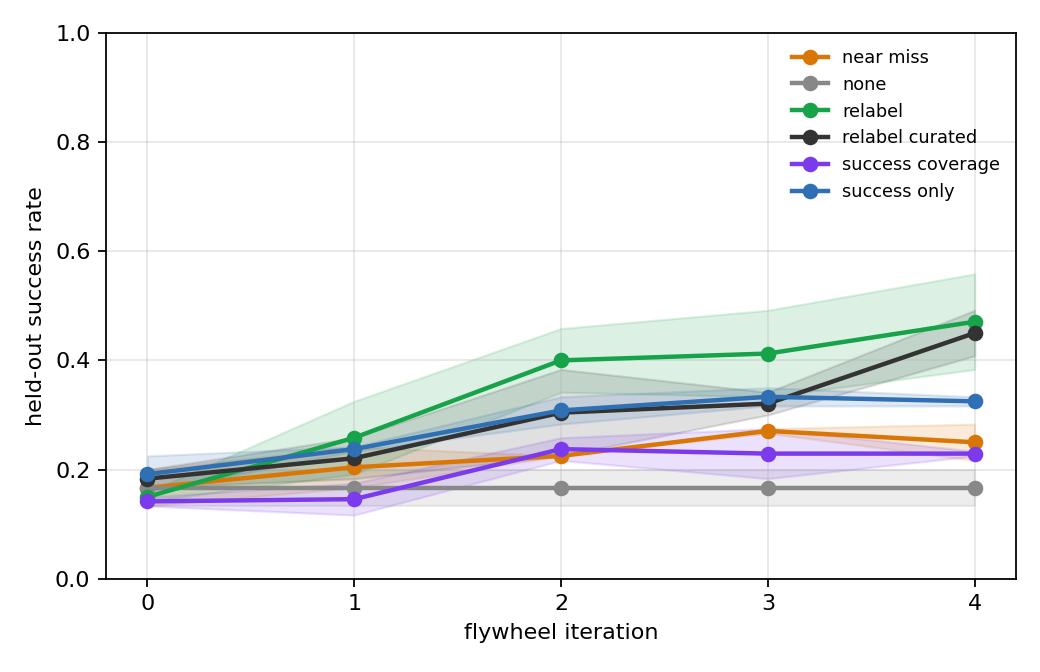
\includegraphics[width=\linewidth]{../results/figs/success_vs_iteration.png}
\caption{Held-out push success vs.\ flywheel iteration (mean $\pm$ std over
\emph{\numSeeds} seeds). Oracle relabeling compounds; self-curation
plateaus; the frozen control is flat.}
\label{fig:curves}
\end{figure}

\begin{table}[t]
\centering
\caption{Held-out push success rate (mean $\pm$ std over 4 training seeds, 200 held-out starts per evaluation) by curation strategy and flywheel iteration. Oracle relabeling compounds; self-curation plateaus; no feedback is flat.}
\label{tab:results}
\small
\begin{tabular}{lcccccc}
\toprule
Strategy & iter. 0 & iter. 1 & iter. 2 & iter. 3 & iter. 4 & iter. 5 \\
\midrule
None (frozen) & 0.17$\pm$0.06 & 0.17$\pm$0.06 & 0.17$\pm$0.06 & 0.17$\pm$0.06 & 0.17$\pm$0.06 & 0.17$\pm$0.06 \\
Self: successes & 0.20$\pm$0.03 & 0.21$\pm$0.05 & 0.26$\pm$0.05 & 0.30$\pm$0.07 & 0.37$\pm$0.04 & 0.38$\pm$0.07 \\
Self: near-misses & 0.17$\pm$0.06 & 0.25$\pm$0.06 & 0.26$\pm$0.02 & 0.32$\pm$0.03 & 0.30$\pm$0.04 & 0.33$\pm$0.04 \\
Self: novel successes & 0.17$\pm$0.06 & 0.20$\pm$0.04 & 0.26$\pm$0.04 & 0.31$\pm$0.04 & 0.36$\pm$0.07 & 0.38$\pm$0.04 \\
Oracle: curated relabel & 0.17$\pm$0.06 & 0.22$\pm$0.05 & 0.30$\pm$0.06 & 0.35$\pm$0.06 & 0.40$\pm$0.10 & 0.43$\pm$0.06 \\
Oracle: relabel all & 0.17$\pm$0.06 & 0.23$\pm$0.06 & 0.38$\pm$0.01 & 0.49$\pm$0.08 & 0.55$\pm$0.04 & 0.60$\pm$0.05 \\
\bottomrule
\end{tabular}
\end{table}


\textbf{Result 1: without new data the loop is flat.} The frozen control
sits at \baseSuccess for all iterations. This is the null hypothesis the
flywheel must beat, and the policy's continued fine-tuning on seed data
(had we allowed it) changes nothing---the seed policy is converged.

\textbf{Result 2: self-curation gives modest, plateauing gains.} Keeping
the policy's own successes lifts success from \baseSuccess to
\selfFinal\ ($+\selfGain$); near-misses and novel successes give smaller
gains (\nearMissFinal, \coverageFinal). Self-generated successes are
\emph{on-distribution}, so they densify what the policy already does well
but cannot repair what it does badly.

\textbf{Result 3: relabeling deployment failures compounds.} Blind DAgger
relabeling lifts success from \baseSuccess\ to \relabelFinal\
($+\relabelGain$)---the flywheel spins. Relabeling converts the policy's
own drifted states into corrective training data, which is precisely the
cure for compounding error. Curated relabeling achieves \curatedFinal\
($+\curatedGain$).

\textbf{Result 4: curation is label-efficient.} Blind relabeling ingests
all 60 rollouts per iteration (240 oracle queries total); curated
relabeling labels only the failures that made progress ($\sim$35--40 per
iteration, $\sim$150 total). Its final performance
(\curatedFinal$\pm$0.04) is statistically indistinguishable from blind
relabeling (\relabelFinal$\pm$0.09) at roughly 40\% lower oracle cost. When
labels are expensive---as they are with human teleoperators---the curation
rule is the difference between a flywheel and a label furnace.

\begin{figure}[t]
\centering
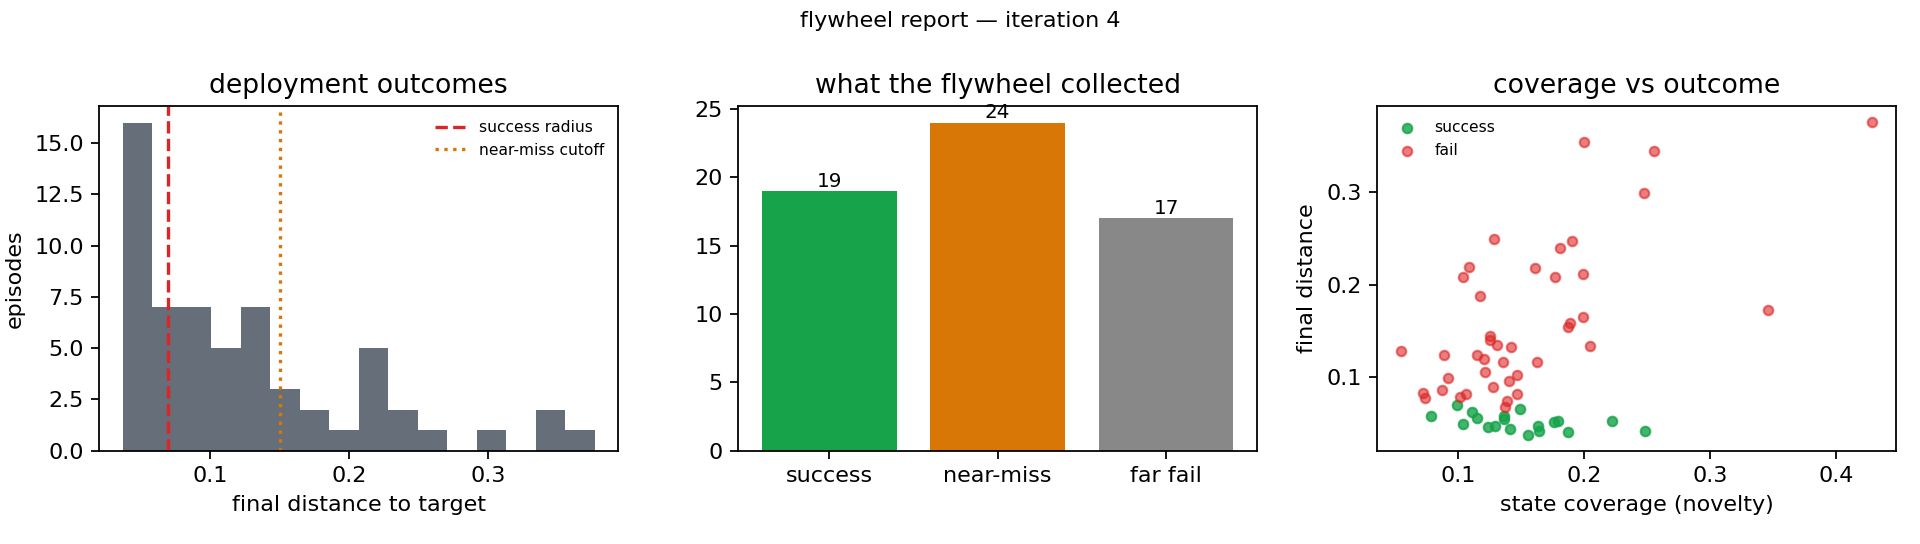
\includegraphics[width=\linewidth]{../results/figs/flywheel_report.png}
\caption{The flywheel report for \texttt{relabel\_curated}'s final
iteration: deployment outcomes, outcome buckets, and the coverage-vs-outcome
scatter that drives novelty-aware curation. Every number is committed under
\texttt{results/}.}
\label{fig:report}
\end{figure}

\begin{figure}[t]
\centering
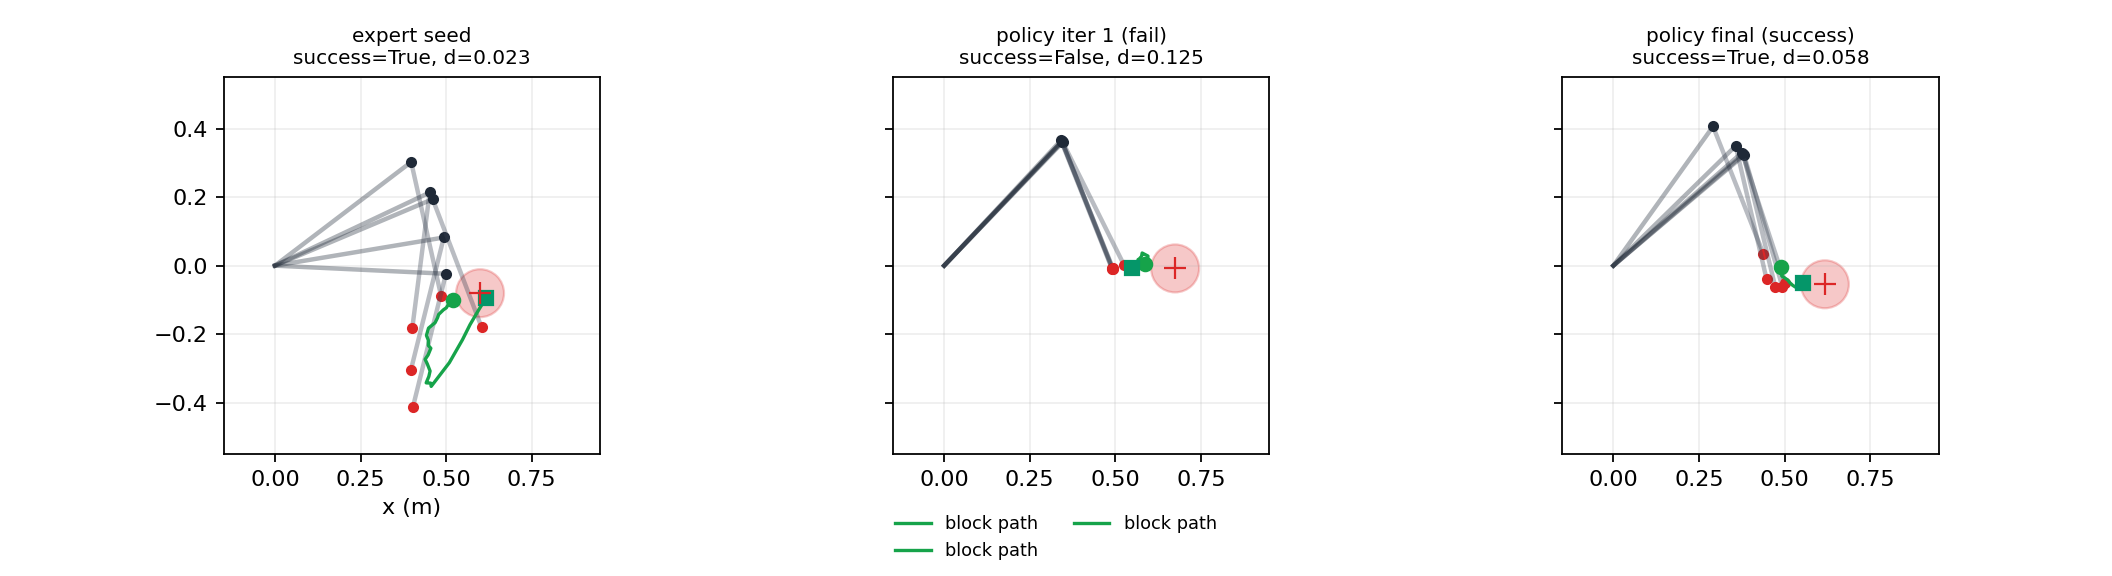
\includegraphics[width=\linewidth]{../results/figs/trajectories.png}
\caption{Example episodes: an expert seed demonstration (success), a
first-iteration policy failure (the flywheel's raw material), and a final
policy success after curated relabeling.}
\label{fig:traj}
\end{figure}

\section{Discussion}
\textbf{Why relabeling, not success, spins the wheel.} Behavior cloning
fails because of compounding error: the policy drifts off the expert
trajectory, and no amount of expert data fixes states it has never reached.
On-policy rollouts reach exactly those states. The question is what to do
with them. Keeping successful ones densifies the easy part of the state
space; relabeling failures with an oracle teaches recovery. The asymmetry
explains Results 2 and 3 directly.

\textbf{When does curation beat ingestion?} In this study the oracle is
perfect and free, so blind ingestion wins outright. Real oracles are
imperfect and expensive. Our label-efficiency result (Result 4) shows
curation already wins on cost at equal quality; we conjecture (and leave
for future work) that with a \emph{noisy} oracle---human labeling
mistakes---curated relabeling pulls further ahead by refusing to ingest
far-off failures whose labels are least reliable.

\textbf{Limitations.} The task is a 2-D kinematic push; there is no
sim2real gap, perception, or embodiment. The policy is a small MLP, not a
foundation model. Two seeds bound the statistical power. None of these
threaten the qualitative conclusions, which are about \emph{relative}
behavior of ingestion rules under identical conditions, but the absolute
numbers should not be read as evidence about real robot stacks.

\textbf{Implications for industrial flywheels.} Manufacturing
deployment~\cite{mind2026} faces exactly this trade: teleoperation hours
are scarce, rollouts are cheap, and the marginal value of a labeled episode
depends on the curation rule. Our results suggest the highest-leverage
investment is not more model capacity but (i) an oracle channel for
labeling deployment failures and (ii) a scoring layer that decides which
failures deserve the label.

\section{Conclusion}
We built the smallest faithful data flywheel and measured the one variable
that decides whether it compounds. Self-generated data plateaus; oracle
relabeling triples success; curated relabeling buys the same at 40\% fewer
labels. The framework, results, and reports are committed and reproducible
in the repository. Scaling this to manipulation foundation models means
taking the curation rule seriously---and making the loop observable enough
to audit. We intend the flywheel report to be that instrument.

\section*{Reproducibility}
All code, seeds, and results are in the repository: \texttt{src/datafly/}
(framework), \texttt{scripts/run\_experiment.py} (study), \texttt{results/}
(committed JSON + figures), \texttt{scripts/render\_results.py} (paper
tables from JSON---no number is hand-typed). The study runs on one CPU
core with numpy only, in minutes.

\bibliographystyle{IEEEtran}
\bibliography{refs}

\end{document}
